\documentclass[12pt,a4paper]{ctexart}

\usepackage[UTF8]{ctex}
\usepackage{geometry}
\usepackage{graphicx}
\usepackage{xcolor}
\usepackage{tikz}
\usepackage{fontspec}
\usepackage{setspace}
\usepackage{enumitem}
\usepackage{booktabs}
\usepackage{array}
\usepackage{longtable}
\usepackage{hyperref}
\usepackage{fancyhdr}
\usepackage{titlesec}
\usepackage{multicol}
\usepackage{xurl}
\usepackage{tocloft}

\renewcommand{\cfttoctitlefont}{\hfill\bfseries\Large}
\renewcommand{\cftaftertoctitle}{\hfill}
\geometry{left=2.5cm,right=2.5cm,top=2.5cm,bottom=2.5cm}

\definecolor{black}{RGB}{0,0,0}
\definecolor{mainblue}{RGB}{0,82,147}
\definecolor{accentgold}{RGB}{180,140,60}
\definecolor{lightgray}{RGB}{245,245,245}
\definecolor{darkgray}{RGB}{80,80,80}
\definecolor{mainred}{RGB}{230,1,45}

\hypersetup{
    colorlinks=true,
    linkcolor=black,
    urlcolor=mainblue,
    citecolor=mainblue,
    pdfborder={0 0 0}
}

\pagestyle{fancy}
\fancyhf{}
\fancyhead[L]{\small\color{darkgray}\textbf{量子行业每周新闻洞察}}
\fancyhead[R]{\small\color{darkgray}\textbf{总第185期}}
\fancyfoot[C]{\thepage}
\renewcommand{\headrulewidth}{0.4pt}
\renewcommand{\footrulewidth}{0pt}

\titleformat{\section}
    {\Large\bfseries\color{mainred}}
    {\thesection、}{0em}{}
\titleformat{\subsection}
    {\large\bfseries\color{mainred}}
    {\thesubsection、}{0em}{}

\newcolumntype{L}[1]{>{\raggedright\arraybackslash}p{#1}}
\newcolumntype{C}[1]{>{\centering\arraybackslash}p{#1}}

\begin{document}

% ==================== 封面 ====================
\begin{titlepage}
\begin{tikzpicture}[remember picture,overlay]
    \fill[mainred] ([yshift=-0.5cm]current page.north west) rectangle ([yshift=-1.2cm]current page.north east);
    \fill[mainred] ([yshift=1.2cm]current page.south west) rectangle ([yshift=0.5cm]current page.south east);
\end{tikzpicture}

\vspace*{4cm}

\begin{center}
    {\fontsize{44}{52}\selectfont\bfseries\color{black} \textbf{量子行业每周新闻洞察}}

    \vspace{0.8cm}

    {\fontsize{16}{22}\selectfont\color{darkgray} 2026.06.20 — 2026.06.26 }
    {\fontsize{16}{22}\selectfont\color{darkgray} \textbf{WEEKLY NEWS}}

    \vspace{1.5cm}

    {\fontsize{20}{26}\selectfont\color{mainred}\textbf{（总第\textbf{ 185 }期）}}

    \vspace{4cm}

    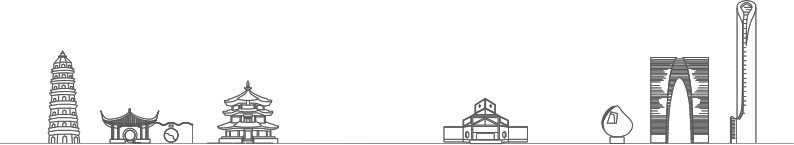
\includegraphics[width=\textwidth]{Cover_Suzhou.png}

    \vfill

    {\fontsize{12}{16}\selectfont\color{darkgray} 量子科技长三角产业创新中心\\编制：战略情报与成果专利室、产业发展部（理事会办公室）}
\end{center}
\end{titlepage}

% ==================== 目录 ====================
\pagenumbering{roman}
\newpage
\tableofcontents

\newpage

% ==================== 摘要 ====================
\pagenumbering{arabic}
\setcounter{page}{1}
\begin{center}
{\Large\bfseries\color{mainred} 摘\hspace{2em}要}
\end{center}
\addcontentsline{toc}{section}{摘要}


\textbf{ 宏观态势：}

全球量子技术竞争步入“体系化部署”新阶段。美国正从军事、立法、基础设施等多维度构建战略护城河，国防部斥资推进量子传感器实战化，立法层面则拟设专门委员会以确保技术领先。与此同时，构建全球量子互联网的设想因卫星地面测试成功而迈出关键一步，首个开放量子网络的启用标志着商业化探索开始与国防战略并行，技术与地缘政治深度捆绑的趋势愈发明显。


\textbf{ 科技前沿：}

量子计算纠错与硬件工程化迎来务实突破。IQM提出的“方向瓷砖码”大幅降低量子比特开销，有望让规模化容错计算更早落地。底层物理研究同样活跃，科学家正通过电场控制电子磁性、利用新型纠缠态抵御噪声，从材料科学和基础物理层面提升量子比特的稳定性。产业界与学术界协作密切，桑迪亚实验室与Quantinuum刷新保真度纪录，标志着软硬件协同优化已成为推动性能飞升的核心路径。


\textbf{ 产品动态：}

量子计算正从“实验室测试”加速迈向“高性能计算融合落地”。Q.ANT的光子处理器以极高能效对标经典计算，标志着量子算力开始在特定场景显露替代潜力。更关键的是，Quandela演示了与英伟达AI基础设施的低延迟集成，橡树岭部署商用机器开启混合量子-HPC生态，这预示着量子已不再是孤立的物理实验，而是作为超级计算架构中的关键加速组件，深度嵌入现有数据与AI工作流。


\textbf{ 企业资讯：}

产业链进入全球布局与生态合纵连横的活跃期。Quantinuum联手慧与科技、Quandela拓展中东市场，显示量子企业正加速融入传统IT与区域科技版图。企业扩张态势明显，Diraq在加州设立新办事处，IQM为上市铺路并引进顶尖高管，表明行业正从纯技术研发向规模化商业运营转型。同时，前政府官员加盟后量子安全公司，凸显了政策与产业在安全领域的高度联动，量子安全商业化进程提速。


\textbf{ 资本运作：}

资本正以前所未有的力度渗透量子计算硬件制造与太空等前沿应用。OQC斥巨资在西班牙建设全球制造中心，Quantum Machines通过收购强化核心硬件构建能力，表明掌控底层制造工艺成为资本布局的焦点。投资视野也在拓宽，INNOSPACE探索太空量子计算，实现了航天与量子的跨界融合。国内初创公司伏曦量子完成天使轮融资，反映出在量子算法领域，中国创新力量正受到资本关注与扶持。




\textbf{ 专利动态：}

本周专利动态涵盖低温环境系统、超导量子测控技术、量子软件与算法共3个板块、14条专利。




% ==================== 会议列表 ====================
{
    \newpage
    \section*{ 7月量子科技行业国内、国际会议}
    \addcontentsline{toc}{section}{ 7月量子科技行业国内、国际会议}
    \scriptsize
    \begin{longtable}{C{0.8cm}L{2.5cm}L{3cm}L{7cm}}
        \toprule[1.5pt]
        \textbf{序号} & \textbf{日期} & \textbf{地点} & \textbf{会议名称} \\
        \midrule
        \endfirsthead
        \toprule
        \textbf{序号} & \textbf{日期} & \textbf{地点} & \textbf{会议名称} \\
        \midrule
        \endhead
        \bottomrule
        \endfoot
        
        1 & 7月1日-3日 & 奥尔堡, 丹麦 & IEEE量子控制、计算与学习国际会议（IEEE qCCL 2026） \\
        \midrule[0.05pt]
        
        2 & 7月1日-3日 & 首尔, 韩国 & 2026量子信息会议（CQI 2026） \\
        \midrule[0.05pt]
        
        3 & 7月1日-3日 & 爱丁堡, 英国 & 2026青年量子研究者暑期学校 \\
        \midrule[0.05pt]
        
        4 & 7月2日-4日 & 首尔, 韩国 & Quantum Korea 2026 \\
        \midrule[0.05pt]
        
        5 & 7月6日-8日 & 海尔布隆, 德国 & 自然科学容错量子计算研讨会（FTQC4NSc） \\
        \midrule[0.05pt]
        
        6 & 7月6日-10日 & 那不勒斯, 意大利 & 第12届单光子研讨会（SPW 2026） \\
        \midrule[0.05pt]
        
        7 & 7月7日-10日 & 加尔各答, 印度 & 2026年IEEE量子计算国际研讨会：电路、系统、自动化与应用（QC-CSAA） \\
        \midrule[0.05pt]
        
        8 & 7月12日-17日 & 马斯特里赫特, 荷兰 & 量子传感与计量学（QSM） \\
        \midrule[0.05pt]
        
        9 & 7月13日-17日 & 代尔夫特, 荷兰 & 第7届自旋量子信息处理会议（Spin Qubit 7） \\
        \midrule[0.05pt]
        
        10 & 7月13日-17日 & 悉尼, 澳大利亚 & IEEE量子软件国际会议（QSW 2026） \\
        \midrule[0.05pt]
        
        11 & 7月16日-18日 & 波尔图, 葡萄牙 & 量子信息、计算、通信与模拟国际会议（QUANTICS 2026） \\
        \midrule[0.05pt]
        
        12 & 7月19日-23日 & 博尔德, 美国 & 有限温度非平衡超流体系统研讨会（FINESS 2026） \\
        \midrule[0.05pt]
        
        13 & 7月20日-24日 & 埃朗根, 德国 & 第30届中欧量子光学研讨会（CEWQO 2026） \\
        \midrule[0.05pt]
        
        14 & 7月22日-23日 & 芝加哥, 美国 & 全球量子论坛（GQF 2026） \\
        \midrule[0.05pt]
        
        15 & 7月25日-26日 & 伊斯顿, 美国 & 量子科学研讨会（Gordon Research Seminar） \\
        \midrule[0.05pt]
        
        16 & 7月26日-31日 & 伊斯顿, 美国 & 多体量子系统：量子计算、模拟、传感与新兴平台（Gordon Research Conference） \\
        \midrule[0.05pt]
        
        17 & 7月26日-8月1日 & 布拉格, 捷克共和国 & 量子与介观热力学前沿2026（FQMT'26） \\
        \midrule[0.05pt]
        
        18 & 7月27日-31日 & 科莫湖, 意大利 & 超快量子光学新前沿暑期学校 \\
        \midrule[0.05pt]
        
        19 & 7月27日-31日 & 艾哈迈达巴德及线上, 印度 & 自由空间量子通信短课程 \\
        \midrule[0.05pt]
        
    \end{longtable}
}




% ==================== 宏观态势 ====================
\newpage
\section{宏观态势}
\vspace{-0.5em}
\noindent\rule{\linewidth}{1.5pt}

\subsection{ 美国国防部启动2亿美元量子传感器计划，加速军事技术革新 }

2026年06月25日消息，美国国防部下属的国防创新单元（DIU）日前宣布启动一项多阶段计划，旨在将成熟的量子传感与授时技术直接转化至联合部队，以支持特朗普总统此前签署的《开启量子创新新前沿》行政令。该计划预计未来一年内投入最高2亿美元，项目重点旨在解决长期困扰军事行动的灵敏度-SWaP（尺寸、重量与功耗）权衡难题。传统的电场、磁场及重力传感器需在高灵敏度、瞬时带宽与SWaP指标之间取舍，而量子技术不受此类限制。项目将围绕四个主要方向展开：电场传感器与磁力计、重力梯度仪、战术时钟以及组件级技术嵌入。相关成果有望为美联合部队提供革命性的情报、监视与侦察能力。

\noindent\textbf{报道链接：}\url{https://www.war.gov/News/Releases/Release/Article/4524344/department-of-war-announces-initiative-to-revolutionize-isr-via-quantum-sensing/}

\subsection{ 波音Q4S量子网络卫星地面测试取得成功，向构建全球量子互联网迈出关键一步 }

2026年06月24日消息，波音公司近日宣布，其Q4S量子网络卫星系统在紧凑型、通过航天认证的有效载荷的地面测试中，成功实现了高保真度的纠缠交换。这一结果标志着在轨验证量子组网技术迈出关键一步。该团队同时完成了环境鉴定测试，以验证该飞行载荷能承受发射应力及太空恶劣环境。随着最终航天器集成工作的启动，Q4S任务仍计划于2027年发射并进行在轨演示。这项里程碑支持了波音构建全球量子互联网的长期愿景，该网络旨在连接远距离的量子传感器与量子计算系统。

\noindent\textbf{报道链接：}\url{https://boeing.mediaroom.com/news-releases-statements?item=131679}

\subsection{ 美国众议员提出新法案，拟设国家量子计算安全委员会以确保技术领先 }

2026年06月23日消息，美国两位众议员近日联合提出一项法案，拟成立独立的国家量子计算安全委员会，以评估美国在量子计算领域的竞争力，并提出政策建议以维持技术领先地位。该拟设委员会由11名成员组成，将审议国家安全、经济竞争力、外国投资、人才培养、研究优先级及量子技术的军事应用等议题。若法案通过，该委员会将从美国国防部获得最高1000万美元拨款，而后需在成立180天内提交首份报告，此后每年将向国会和美国总统提出建议，并持续运作至2030年10月1日。

\noindent\textbf{报道链接：}\url{https://thequantuminsider.com/2026/06/18/u-s-lawmakers-introduce-bill-to-create-national-quantum-security-commission/}

\subsection{ 美国首个开放量子网络在新墨西哥州启用，将助推商业化量子技术发展 }

2026年06月20日消息，量子网络公司Qunnect今年2月底已在新墨西哥州正式启用了美国首个开放接入的、基于纠缠的量子网络ABQ-Net。目前该网络已通过商用光纤互联两个节点，分别是Qunnect位于阿尔伯克基市中心的办公室，以及由桑迪亚国家实验室和洛斯阿拉莫斯国家实验室运营的综合纳米技术中心。波士顿量子网络软件公司Aliro Quantum是首批用户之一，它正基于该网络提供量子安全服务。据悉，ABQ-Net由Roadrunner Venture Studios提供资助，并得到新墨西哥州经济发展部的支持，是新墨西哥州投入逾3亿美元打造量子经济计划的一部分。

\noindent\textbf{报道链接：}\url{https://www.qunnect.inc/press-releases/2026-02-24}


% ==================== 科技前沿 ====================
\newpage
\section{科技前沿}
\vspace{-0.5em}
\noindent\rule{\linewidth}{1.5pt}

\subsection{ 量子计算机公司IQM发布“方向瓷砖码”，量子比特开销可减少1000倍 }

2026年06月25日消息，IQM量子计算机公司近日宣布在量子纠错领域取得重要进展，它通过引入“方向瓷砖码（directional tile codes）”这一新型纠错码家族，朝着实用化、大规模容错量子计算迈出关键一步。该研究表明，仅利用IQM Crystal处理器中已有的最近邻iSWAP门，该纠错码便能在每个逻辑量子比特约30个物理量子比特的硬件规模下，将每轮每个逻辑量子比特的错误率相比广泛使用的表面码降低多达1000倍。研究成果已在arXiv预印本平台发布，由IQM与柏林自由大学、爱丁堡大学及美因茨大学的研究人员合作完成。

\noindent\textbf{报道链接：}\url{https://iqm.tech/press-releases/iqm-achieves-milestone-in-quantum-error-correction-enabling-fault-tolerant-computing-in-the-near-term/}

\subsection{ Sarborg获得纽约私募基金投资，启动量子部门SarborgQ }

2026年06月25日消息，Sarborg Limited近日完成了一轮来自纽约私人投资基金的融资。该轮融资每股认购价为12.5万美元，对应完全稀释估值约6.383亿美元。Sarborg表示，募集资金将用于支持其新成立的量子计算部门SarborgQ的启动与开发，同时推动自有数据集扩展、知识产权加速生成、资产开发活动以及Sarborg Signature Agent和AI平台的进一步发展。SarborgQ将专注于将量子计算应用于现有的Signature Intelligence平台，旨在增强对复杂生物系统的分析能力、改进因果推断，并在多维数据集中生成更高分辨率的签名。

\noindent\textbf{报道链接：}\url{https://www.globenewswire.com/news-release/2026/06/18/3314166/0/en/cdt-notes-strategic-investment-into-sarborg-and-expansion-into-quantum-computing.html}

\subsection{ 麻省理工研发出新型柔性低温电缆，Maybell Quantum已获得其设计许可 }

2026年06月23日消息，麻省理工学院林肯实验室的研究人员研发出一种柔性带状低频电缆原型，这种电缆不仅满足稀释制冷机所需的极低温环境、保持高效直流供电并支持高速数据传输的布线系统，而且还与商用电路板制造工艺兼容。据悉，量子低温系统开发商Maybell Quantum已获得该电缆的设计许可，并将把其适配于自家稀释制冷机。

\noindent\textbf{报道链接：}\url{https://www.ll.mit.edu/news/flexible-cryogenic-cables-solve-challenge-quantum-system-development}

\subsection{ 北京理工大学在石墨烯莫尔条纹系统中的量子霍尔效应研究方面取得进展 }

2026年06月23日消息，北京理工大学的研究人员近日在《物理评论快报》上发表一项研究，他们发现了一种全新类型的量子振荡，这种振荡源于石墨烯莫尔条纹系统中的非线性霍尔效应。他们利用相互扭曲堆叠的单层石墨烯材料发现，当外加磁场周期性变化时，电子会重组为新型量子态，且这些态由奇异准粒子主导，表现得如同周围的磁场仿佛被“关闭”。他们实验发现，该材料中的非线性霍尔信号会随着这些周期性出现的条件同步振荡。该成果不仅确立了一种新型量子振荡，还为探测奇异物质相提供了全新路径。

\noindent\textbf{报道链接：}\url{https://phys.org/news/2026-06-quantum-hall-effect-gains-graphene.html}

\subsection{ 智能光镊系统SmartTrap问世，无需人工干预且效率得到大幅提升 }

2026年06月23日消息，瑞典哥德堡大学的研究人员与合作者合作开发出一款名为SmartTrap的AI系统，这是一种能够加快光镊操作的人工智能系统。据介绍，SmartTrap系统能够自主完成颗粒捕获、数据测量及新样本加载，全程无需人工干预。在多项严格测试中：该AI平台每小时可分类与表征数百个颗粒；在生物物理学领域技术要求最高的单分子DNA拉伸实验中，该系统每小时可执行10至15次实验。此外，SmartTrap还成功实现了红细胞机械刚度的测定，并绘制了不同盐浓度下颗粒对之间纳米级静电力图。

\noindent\textbf{报道链接：}\url{https://www.gu.se/en/news/ai-speed-up-the-use-of-optical-tweezers}

\subsection{ 新研究表明可通过电场精确控制石墨烯中电子的磁性行为 }

2026年06月23日消息，英国曼彻斯特大学石墨烯实验室与新加坡国立大学的研究人员近日在《自然通讯》上发表一项研究，证明可通过电场精确控制石墨烯中电子的磁性行为，并在精心设计的石墨烯系统中观测到异常大的自旋信号。该研究展示了将石墨烯置于磁性材料附近时，无需永久改变石墨烯本身即可影响电子自旋。这种强大的信号出现在一个旨在打开电子结构能隙的双层石墨烯超晶格器件中，该器件测得自旋极化率接近50\%，非局域自旋电阻超过300欧姆。研究人员表示，该成果有望为基于石墨烯的自旋电子学提供新的调控手段。

\noindent\textbf{报道链接：}\url{https://phys.org/news/2026-06-electrically-tunable-polarization-graphene-path.html}

\subsection{ 科学家利用新型量子纠缠态来帮助量子传感器抵御环境噪声 }

2026年06月22日消息，一组国际科研团队提出一种新型纠缠态，它可帮助量子传感器有效抑制环境噪声。这种纠缠态利用了无消相干子空间，这些子空间可免受某些类型的干扰，从而抑制影响两个传感器的噪声。该团队通过构建“自旋交换”机制，使传感器网络的两个节点相互纠缠，其中一个节点中的每个原子都与另一个中的每个原子完全反相关。利用该方法，他们可实现海森堡标度，从而实现最佳测量精度。相关成果已于近日发表在《物理评论X》期刊。

\noindent\textbf{报道链接：}\url{https://www.colorado.edu/physics/2026/06/10/new-kind-entanglement-helps-quantum-sensors-tune-out-noise}

\subsection{ 桑迪亚实验室与Quantinuum合作测试Helios系统性能 保真度再创新纪录 }

2026年06月21日消息，美国桑迪亚国家实验室与量子计算公司Quantinuum近日在《自然》杂志联合发表一篇论文，报告了Quantinuum于去年推出的98量子比特商用系统Helios的性能表现。测试显示，该系统在单量子比特和双量子比特操作中，保真度分别达到99.9975\%和99.921\%，创下该公司迄今规模最大、可靠性最高的量子计算机纪录。这一成果标志着美国能源部在实现容错量子计算目标方面取得稳步进展。

\noindent\textbf{报道链接：}\url{https://newsreleases.sandia.gov/in-the-mountain-west-a-quantum-computing-collaboration-announces-major-results/}


% ==================== 产品动态 ====================
\newpage
\section{产品动态}
\vspace{-0.5em}
\noindent\rule{\linewidth}{1.5pt}

\subsection{ Q.ANT第二代NPU亮相ISC高性能计算大会，其光子架构能效是经典处理器30倍 }

2026年06月25日消息，Q.ANT公司在近日于汉堡举办的ISC High Performance 2026大会上，成功在其第二代原生处理单元（NPU）上演示了扩散模型和循环神经网络。Q.ANT还运行了由奥地利前沿AI实验室NXAI开发的TiRex时间序列预测模型。这证明Q.ANT的光子架构能够支撑生成式图像合成与时序预测等现代AI能力的全范围应用。Q.ANT表示，基于其硬件，这些高性能计算任务在光子电路层面的等效矩阵运算中，能效目标有望达到经典处理器的30倍。

\noindent\textbf{报道链接：}\url{https://qant.com/press-releases/q-ant-runs-generative-ai-on-photonic-hardware/}

\subsection{ Quandela成功演示光子量子处理器与英伟达AI基础设施间的低延迟集成 }

2026年06月25日消息，法国光量子计算公司Quandela近日宣布，它已实验验证一条光子量子处理器与英伟达AI基础设施间的低延迟集成路径，这标志着向将量子处理单元直接引入高性能计算环境迈出了重要一步。具体验证显示，Quandela的光子量子处理单元可通过英伟达NVQLink与英伟达GPU主机及基于FPGA的量子系统控制器协同工作。这一成果支持了一种新的混合量子-经典计算执行模式：从远程量子接入转向HPC基础设施内部共置量子加速。

\noindent\textbf{报道链接：}\url{https://www.quandela.com/newsroom-posts/quandela-photonic-qpu-nvidia-hpc-integration/}

\subsection{ D-Wave推出首款专为错误感知编程而打造的门模型量子计算模拟器 }

2026年06月23日消息，D-Wave Quantum近日宣布，它将推出其首款专为错误感知编程而设计的门模型量子计算模拟器。D-Wave此次推出的模拟器基于其双轨技术构建，能够实时检测并反馈处理器运行中的错误，使开发者能够根据真实硬件行为设计更具弹性的量子应用和工作流程。该模拟器通过结合错误检测与实时控制，能为开发者提供理解量子行为、构建量子应用及纠错程序原型、探索高级工作流的新工具和数据。

\noindent\textbf{报道链接：}\url{https://www.dwavequantum.com/company/newsroom/press-release/d-wave-announces-world-s-first-gate-model-quantum-computing-simulator-for-error-aware-programming/}

\subsection{ QTREX Quantum利用其单体构建AME工艺成功生产出低温芯片载具 }

2026年06月23日消息，QTREX Quantum近日宣布实现一项重要技术与战略里程碑：该公司已采用其专有的单体构建AME（增材制造电子）工艺，成功生产出一款低温芯片载具。该设计由一家知名的美国全栈量子计算系统开发商提供。据悉，单体构建AME工艺旨在将低温芯片载具与互连结构集成于单一整体架构中，使导电通道、介电结构、屏蔽功能及直接互连部件得以一次成型，无需通过分离连接器和人工步骤进行组装。这一成果将QTREX在量子硬件堆栈中的角色扩展至处理器-接口层，表明其AME平台能在量子处理器周围同时处理信号传输和关键载波级功能。

\noindent\textbf{报道链接：}\url{https://www.globenewswire.com/news-release/2026/06/18/3314085/0/en/qtrex-expands-into-quantum-processor-interface-with-single-build-cryogenic-chip-carrier.html}

\subsection{ 橡树岭实验室部署首台商用量子计算机，将开启混合量子-HPC新生态 }

2026年06月22日消息，美国橡树岭国家实验室（ORNL）近日正式启用了其采购的首台商用量子计算机“Pathfinder”，该设备由IQM量子计算公司制造并部署。这台20量子比特的IQM Radiance系统也是IQM在美国安装的首台量子计算机。目前，Pathfinder已接入美国国家计算科学中心技术集成小组测试平台的HPC系统，ORNL研究人员将利用它开发混合量子-HPC生态系统的相关方法与工具。

\noindent\textbf{报道链接：}\url{http://iqm.tech/press-releases/iqm-deploys-its-first-u-s-quantum-computer-at-oak-ridge-national-laboratory/}

\subsection{ 瑞士网络安全公司DuoKey推出量子风险评分服务 }

2026年06月22日消息，瑞士网络安全公司DuoKey近日推出了量子风险评分（Quantum Risk Score）服务，旨在帮助企业在后量子密码迁移中明确优先行动方向。该服务是一种结构化的密码学评估工具，它通过分析企业可观测的域名暴露面，对照当前后量子标准生成0至100的综合指数，它无需访问内部系统，仅依赖公开信号，因此很容易快速部署。其评估报告包含完整的密码资产清单、优先级迁移矩阵、针对NIST、CNSA 2.0、NCSC、ANSSI和BSI框架的合规差距分析，以及一份为期36个月的迁移路线图。

\noindent\textbf{报道链接：}\url{https://www.prnewswire.com/news-releases/duokey-launches-quantum-risk-score-to-help-enterprises-prioritise-post-quantum-cryptography-migration-302803366.html}

\subsection{ IonQ推出Clavis XG Multiplex，可使量子安全技术能在城域网中大规模部署 }

2026年06月20日，IonQ发布其旗下ID Quantique公司Clavis XG量子密钥分发（QKD）产品组合的新成员——Clavis XG Multiplex，旨在提升量子安全技术在城域光纤网络中的实用性和部署便利性。该产品支持在同一城域光纤基础设施上实现量子与经典通信共存，无需运营商重新设计、隔离或专用光网络，从而提供低成本方案，可在企业进行后量子密码（PQC）迁移的同时，对敏感数据和高风险网络段直接降低长期密码风险。IonQ表示，Clavis XG Multiplex允许客户在同一光纤上传输多种数据类型，提升IonQ量子安全平台的性能，使现有基础设施更具企业级安全性，并降低了QKD的运营成本。

\noindent\textbf{报道链接：}\url{https://www.ionq.com/news/ionq-introduces-clavis-xg-multiplex-making-quantum-security-deployable-at-scale-in-metro-networks}



% ==================== 专利动态 ====================
\newpage
\section{专利动态}
\vspace{-0.5em}
\noindent\rule{\linewidth}{1.5pt}

\subsection{ 低温环境系统 }

\subsubsection{ 一种多端口频分复用滤波器 }

申请人：清华大学 | 无锡东微量子科技有限公司

发明人：戴根婷 | 杨亮亮 | 何楷泳 | 耿霄 | 程明俊 | 陈国动 | 孟范忠 | 陈宏江 | 刘建设 | 陈炜

公开日/授权日：2026-06-23

摘要：

本申请公开了一种多端口频分复用滤波器，包括：一个或一个以上选频滤波模块，每个所述选频滤波模块设置一个输入端口，一个或一个以上输出端口；每个所述选频滤波模块包括：一个或一个以上耦合模块、一个或一个以上不同频率的谐振腔；耦合模块，用于将经由输入端口输入的一段频率信号耦合到不同频率的谐振腔；谐振腔，用于完成对应频率信号的选择性传递，并从对应的输出端口输出。通过本申请实施例实现了可调频段的单腔体带通滤波功能。不仅能解决超导量子计算领域中XY控制线端口复用的问题，而且具备在其他应用领域实现多段式频分复用功能的潜力，突破对于推动量子处理器的规模化扩展具有重大意义。

\noindent\textbf{专利链接：}\url{https://analytics.zhihuiya.com/patent-view/abst?patentId=843949ff-4186-4691-b320-a19f523d5d73&shareId=193FC1D0-D471-7F90-B17C-E5CE67738GC2&from=EXPORT&signature=aJUzGZXrbtcmlPQp886n88Uh40i65wr%2FbHJRscldW9s%3D&expire=94608000&date=20260626T004136Z&version=1.0}

\subsubsection{ 集成式量子比特输出链路 }

申请人：相干(北京)科技有限公司

发明人：赵剑琴

公开日/授权日：2026-06-23

摘要：

本申请提出了一种集成式量子比特输出链路，涉及输入/输出装置的链路技术领域。本申请所要解决的问题是，量子比特传输时，空间受限，难以实现高效的热处理。本申请提出的集成式量子比特输出链路，包括：三节环形器；负载，负载设置在三节环形器上，负载用于吸收反向传输的信号；约瑟夫森参量放大器，约瑟夫森参量放大器内置有连接器，约瑟夫森参量放大器通过连接器连接三节环形器。本实用新型提出的集成式量子比特输出链路，使得量子比特可以在超级低温环境下依然保持良好的性能，达到了高集成、高导热和磁屏蔽的效果，并且易于装配和大批量生产，有效减小集成式量子比特输出链路的体积。

\noindent\textbf{专利链接：}\url{https://analytics.zhihuiya.com/patent-view/abst?patentId=71a205ba-d0c8-4143-9495-276d9dffd4d6&shareId=193FC1D0-D471-7F90-B17C-E5CE67738GC2&from=EXPORT&signature=8rAQrUaJLOyh3l%2FNaVcvS71ZGhvTwJzCRWQdo0zECAw%3D&expire=94608000&date=20260626T004136Z&version=1.0}

\subsubsection{ 利用石墨烯的基于卡西米尔效应的隧道晶体管 }

申请人：QUBIT SEMICONDUCTOR LLC

发明人：DANNEMILLER, DOUGLAS JOSEPH

公开日/授权日：2026-06-23

摘要：

一种量子器件包括:致动器,其包含石墨烯材料,且近端安装于致动器锚点;电极,其位于致动器的远端;量子点,其配置用于局域单个电子,该量子点和电极位于同一真空中以形成隧穿间隙;以及量子点锚点,其包含石墨烯材料,相对于电极与量子点位于同一平面。该量子器件可包括调制器,其配置用于发射特定频率范围内的电磁信号。石墨烯材料被调谐以响应电磁信号而增强电极和量子点锚点之间的卡西米尔力。增强的卡西米尔力使致动器发生形变,从而使电极进入量子点的电子隧穿范围,或者降低静态电极上的隧穿势垒。

\noindent\textbf{专利链接：}\url{https://analytics.zhihuiya.com/patent-view/abst?patentId=78e78df7-d44b-4d39-9591-c546be0473f8&shareId=193FC1D0-D471-7F90-B17C-E5CE67738GC2&from=EXPORT&signature=kEqkH37DeThYozUBJyinFYrTEiUZpx1LUXH3yFZeneU%3D&expire=94608000&date=20260626T004136Z&version=1.0}

\subsubsection{ 包含量子电容器的参数放大器 }

申请人：微软技术许可有限责任公司

发明人：萊利 大衛J

公开日/授权日：2026-06-21

摘要：

描述了与包括量子电容器的参数放大器有关的系统及方法。在一个实例中,提供了包含用于接收量子位元信号的输入端子的参数放大器。参数放大器进一步包括用于接收泵送信号的泵送端子。参数放大器进一步包含放大器,该放大器包括复数个量子电容装置,该复数个量子电容装置经配置以在低温环境中操作,并经配置以借由将量子位元信号与泵送信号混合以产生放大信号来放大量子位元信号。参数放大器进一步包括用于提供放大信号的输出端子。

\noindent\textbf{专利链接：}\url{https://analytics.zhihuiya.com/patent-view/abst?patentId=a933b1a4-1ee7-4584-8654-0684310adaba&shareId=193FC1D0-D471-7F90-B17C-E5CE67738GC2&from=EXPORT&signature=6jWGghLF01f49p61BaiFOq9zGIxcB5bNew4wkAPdLaI%3D&expire=94608000&date=20260626T004136Z&version=1.0}


\subsection{ 超导量子测控技术 }

\subsubsection{ 用于量子数据查找的电路设计 }

申请人：微软技术许可有限责任公司

发明人：SUNDARAM, AARTHI MEENAKSHI | ZHU, SHUCHEN | LOW, GUANG HAO

公开日/授权日：2026-06-24

摘要：

本公开的方面包括一种量子查找技术。这些方面包括:响应于接收输入,将输入路由通过第一量子路由器以确定第一输出。这些方面包括:将第一输出路由到至少一个第二量子路由器,该至少一个第二量子路由器将第一输出馈送到门树,该门树生成第二输出,该第二输出被馈送到量子位,量子位执行操作并生成读出。这些方面包括:将读出路由通过第三量子路由器,该第三量子路由器被布置用于输出读出。

\noindent\textbf{专利链接：}\url{https://analytics.zhihuiya.com/patent-view/abst?patentId=b499c2e1-f153-4f19-a7e8-6ee31a3a32cf&shareId=4G0297G6-613E-5D50-0F19-1180B5GF30B6&from=EXPORT&signature=FjmTR%2Ftxl92ABHSVId64caGwZfwno5i3ahDj%2FpWgmLQ%3D&expire=94608000&date=20260626T004457Z&version=1.0}

\subsubsection{ 使用超导刚挠电路支持量子位平面与量子位平面的控制系统之间的高热梯度的系统和方法 }

申请人：微软技术许可有限责任公司

发明人：TURNER, MATTHEW DAVID | RANTA, CRAIG STEVEN | KRAMER, KEVIN JAMES

公开日/授权日：2026-06-24

摘要：

本文描述了用于在量子比特平面和该量子比特平面的控制系统之间维持高温度梯度的系统和方法。该系统包括与超导刚挠性电路的第一刚性电路部分关联的量子比特平面,以及与该超导刚挠性电路的第二刚性电路部分关联的控制系统。该超导刚挠性电路包括用于连接第一刚性电路部分和第二刚性电路部分的柔性电路部分。该系统还包括第一冷却系统,用于将量子比特平面和超导刚挠性电路的第一刚性电路部分的工作温度维持在100毫开尔文或以下。该系统还包括第二冷却系统,用于将控制系统和超导刚挠性电路的第二刚性电路部分的工作温度维持在10开尔文或以下。

\noindent\textbf{专利链接：}\url{https://analytics.zhihuiya.com/patent-view/abst?patentId=1f47e0c7-88cb-480e-a7ae-4febb8a3e7ff&shareId=4G0297G6-613E-5D50-0F19-1180B5GF30B6&from=EXPORT&signature=8EIoDq3OQi8gSMy%2FjYxsGCrcMLVQY7Uzb9K8gG6gugU%3D&expire=94608000&date=20260626T004457Z&version=1.0}


\subsection{ 量子软件与算法 }

\subsubsection{ 系统 }

申请人：软银集团股份有限公司

发明人：北山 翔平

公开日/授权日：2026-06-22

摘要：

我们提供系统。 

 [解决方案] 

一种利用放置在家庭环境中的录音设备来收集儿童行为信息的方法, 

一种利用智能模型分析已收集到的各种信息来评估儿童发展特征的方法; 

根据评估结果,提出一种促进儿童教育和发展的建议方法, 

一种分析儿童情绪状态并根据需要提供即时报告的方法, 

一种通过持续的数据积累来预测发育模式并及早发现潜在发育挑战的方法, 

一种利用移动自主设备监测儿童活动并提供互动式教育体验的方法, 

该系统包括根据分析结果向家长提供即时反馈并推荐个性化育儿方法的手段。

\noindent\textbf{专利链接：}\url{https://analytics.zhihuiya.com/patent-view/abst?patentId=f36cf315-d771-4bd4-bd79-851b2461e788&shareId=198G292E-EE74-750G-3C47-5E63C2EB5B01&from=EXPORT&signature=aPG1NpV1V4CDLw5vBIOMLwos9FU5AfJFQu6bhMP%2BD9c%3D&expire=94608000&date=20260626T004645Z&version=1.0}

\subsubsection{ 系统 }

申请人：软银集团股份有限公司

发明人：鈴木 貴雄

公开日/授权日：2026-06-24

摘要：

我们提供系统。 

 [解决方案] 

收集和分析多语言信息的方法, 

一种利用生成算法设计新的标准表示的方法, 

将多语言信息转换为标准化表达并进行压缩的方法

一种利用转换后的信息优化预测模型的方法, 

一种利用预测模型与用户进行双向通信的方法, 

一种实时呈现翻译信息的方式, 

包含此功能的系统。

\noindent\textbf{专利链接：}\url{https://analytics.zhihuiya.com/patent-view/abst?patentId=05206804-f180-4003-a513-4128990ff3d7&shareId=198G292E-EE74-750G-3C47-5E63C2EB5B01&from=EXPORT&signature=mX%2F6Si8MtE3gzweHffnMsOY2wPMMXXMimxAnhfRn2dk%3D&expire=94608000&date=20260626T004645Z&version=1.0}

\subsubsection{ 制造量子器件的方法 }

申请人：富士通株式会社

发明人：MIYATAKE, TETSUYA

公开日/授权日：2026-06-24

摘要：

一种制造量子器件(100、200)的方法,包括:将包括色心(21)的金刚石衬底(30)键合到设置在支撑衬底(10)上的层(32);在键合金刚石衬底之后,通过蚀刻金刚石衬底形成包括色心的第一部分(40)和具有相对于第一部分的侧壁(41)倾斜的倾斜表面(43)的第二部分(42);在倾斜表面上形成金属膜(45);以及通过将由金属膜反射的激光束发射到第一部分的侧壁上,在比色心更远离层的第一位置处切割第一部分,形成第一光波导部分(20)。

\noindent\textbf{专利链接：}\url{https://analytics.zhihuiya.com/patent-view/abst?patentId=147d295d-d8ec-42f5-992e-6849a8347ea5&shareId=198G292E-EE74-750G-3C47-5E63C2EB5B01&from=EXPORT&signature=1LRVFVPrGAVE63BzDm9n2Gd4dL4mu06NQBSQPD7%2FE3s%3D&expire=94608000&date=20260626T004645Z&version=1.0}

\subsubsection{ 将应用迁移到后量子密码术(PQC)状态的工作量的估计 }

申请人：塔塔顾问服务有限公司

发明人：BHOWMICK, AMIT | VIDHANI, KUMAR MANSUKHLAL | ALASINGARA, BHATTACHAR

公开日/授权日：2026-06-24

摘要：

过去几十年来,准确估计完成应用迁移所需的代码行(LoC)的能力一直是一个挑战。本文公开的实施例提供了一种用于估计将应用迁移到后量子密码(PQC)状态的工作量的方法和系统。基于针对存在于精细分片输出和精细耦合输出中的一个或多个组件所确定的循环复杂度来估计该系统。此外,使用循环复杂度和受一个或多个密码API影响的LoC的数量来估计迁移的工作量。

\noindent\textbf{专利链接：}\url{https://analytics.zhihuiya.com/patent-view/abst?patentId=33c6710b-c21a-4984-bbe8-048106c16b2b&shareId=198G292E-EE74-750G-3C47-5E63C2EB5B01&from=EXPORT&signature=Wap4suo%2BlI8eezOxtgJgww9rFAJGRuV8FW%2FcLrGzzts%3D&expire=94608000&date=20260626T004645Z&version=1.0}

\subsubsection{ 减少量子计算机中使用的量子位 }

申请人：微软技术许可有限责任公司

发明人：SU, YUAN | KANG, CHRISTOPHER THOMAS

公开日/授权日：2026-06-24

摘要：

本公开的各方面包括用于操作量子电路的过程。各方面包括利用单元演化对第一被乘数和第二被乘数执行哈密尔顿块编码,分别产生第一中间算子和第二中间算子。各方面包括对第一中间算子执行第一门和对第二中间算子执行第二门,分别产生修改的第一中间算子和修改的第二中间算子。各方面包括执行交换子积公式以组合修改的第一中间算子和修改的第二中间算子,产生组合算子,并且对组合算子执行另一第一门和另一第二门,产生修改的组合算子。另一第二门包括另一第一门的共轭转置。在量子电路上利用两个辅助量子位。

\noindent\textbf{专利链接：}\url{https://analytics.zhihuiya.com/patent-view/abst?patentId=99cacae8-3277-48aa-bcd5-40b7bc9556c9&shareId=198G292E-EE74-750G-3C47-5E63C2EB5B01&from=EXPORT&signature=HRm5nYt9eqUsmWz0RhgB6gBmUNjJzwQKKPPJWB%2BP1zQ%3D&expire=94608000&date=20260626T004645Z&version=1.0}

\subsubsection{ 量子点阵列的制造和有效接触各种栅极的方式 }

申请人：原子能和替代能源委员会

发明人：BERTRAND, BENOIT

公开日/授权日：2026-06-24

摘要：

量子电子器件包括:- 用于容纳量子点的活性区域 (20),以及,- 紧贴该器件一个表面的:a) 多条网格线 (G11、G12、G13、G14),这些网格线彼此电隔离,并且每条网格线覆盖活性区域 (20) 的一部分;以及 b) 重建促进岛 (14-17、I4a-I7a),每条网格线上至少有一个岛,重建促进岛彼此间隔距离 (D1、D2、D3),每个重建促进岛包括一个侧翼,网格线的侧部 (P4-P7) 沿该侧翼延伸,该器件还包括至少一个电触点 (P4-P7),用于接触至少一条给定的网格线 (G11、G12、G13、G14)。至少一个电触点位于沿触点重建促进岛侧边延伸的给定网格线的侧面上(14-17,I4a-I7a)。

\noindent\textbf{专利链接：}\url{https://analytics.zhihuiya.com/patent-view/abst?patentId=92bb9f73-0f44-40dc-b3b6-f7273088bdf1&shareId=198G292E-EE74-750G-3C47-5E63C2EB5B01&from=EXPORT&signature=uBapswM4SNm755iLb%2FLWAbPS5zRkhGk5%2FKk2ude%2F9L4%3D&expire=94608000&date=20260626T004645Z&version=1.0}

\subsubsection{ 系统 }

申请人：软银集团股份有限公司

发明人：五條 眞樹

公开日/授权日：2026-06-24

摘要：

我们提供系统。 

 [解决方案] 

为了支持跨文化交流, 

收集不同文化信息的方法

一种利用自然语言处理技术分析用户输入以了解文化背景的方法

一种根据分析结果制定合适的沟通策略的方法, 

向用户展示生成策略的一种方式, 

基于乘客文化背景的语音导览优化方法

包含此功能的系统。

\noindent\textbf{专利链接：}\url{https://analytics.zhihuiya.com/patent-view/abst?patentId=6db73478-fd06-4259-907b-029fbe6fe32e&shareId=198G292E-EE74-750G-3C47-5E63C2EB5B01&from=EXPORT&signature=goKIEMdPH0oyF7LWIV6ShkWi2LLkDhTR3t6KZbRyaAE%3D&expire=94608000&date=20260626T004645Z&version=1.0}

\subsubsection{ 系统 }

申请人：软银集团股份有限公司

发明人：松崎 達彦

公开日/授权日：2026-06-24

摘要：

我们提供系统。 

 [解决方案] 

一种利用自然语言处理算法分析电子邮件正文,并从中提取预定信息元素的方法; 

一种基于提取的信息元素自动生成电子邮件主题行的方法, 

一种利用生成式人工智能模型生成与电子支付等事件相关的电子邮件主题行的方法, 

一种在移动信息终端设备的用户界面上显示生成的电子邮件主题的方法, 

包含此功能的系统。

\noindent\textbf{专利链接：}\url{https://analytics.zhihuiya.com/patent-view/abst?patentId=61040822-06cc-4bc7-ac72-f5d29ba20241&shareId=198G292E-EE74-750G-3C47-5E63C2EB5B01&from=EXPORT&signature=GmrQFBGaBjPoMklYAlWW6mwoDp5U6B97cTe2leqt55A%3D&expire=94608000&date=20260626T004645Z&version=1.0}




% ==================== 企业资讯 ====================
\newpage
\section{企业资讯}
\vspace{-0.5em}
\noindent\rule{\linewidth}{1.5pt}

\subsection{ PTG与PolarisQB签署独家代理协议，加速后者量子药物发现平台落地 }

2026年06月24日消息，POLARISQB科技集团（简称PTG）与PolarisQB近日宣布签署一项覆盖大中华区及东南亚市场的独家代理协议。根据协议，PTG将成为PolarisQB在中国大陆、香港、澳门、台湾以及东盟十国的独家代表。此举旨在将PolarisQB基于量子计算的药物发现平台QuADD推向全球增长最快的生物制药市场之一。据悉，QuADD利用量子退火和量子启发算法，可在数小时内探索高达10\textasciicircum{}30量级的候选分子空间，并优化结合亲和性、成药性和合成可行性等多参数目标。

\noindent\textbf{报道链接：}\url{https://polarisqb.com/polaris-news/ptg-and-polarisqb-announce-exclusive-representation-agreement-for-greater-china-and-southeast-asia/}

\subsection{ EPB Quantum将于10月初在美国田纳西州举办首届量子商业会议 }

2026年06月24日消息，美国田纳西州查塔努加市将于2026年10月1日举办首届“量子商业（QiB）”会议，由EPB Quantum主办。会议将聚焦量子计算如何在金融、医疗、保险、化工、物流及汽车等领域，为企业带来经济价值，并帮助商业和技术领导者把握先机。

\noindent\textbf{报道链接：}\url{https://epb.com/newsroom/press-releases/epb-quantum-hosts-conference/}

\subsection{ 前美国国会及国防部官员加盟BTQ，出任后量子安全战略顾问 }

2026年06月25日消息，BTQ Technologies近日宣布任命Brandt Pasco为后量子密码与安全领域的美国战略顾问，他将负责推动BTQ与美国政府利益相关方、公共部门机构、研究机构、国家安全组织及战略产业伙伴的沟通协作。BTQ表示，Pasco拥有超过二十年的政府、法律、私募股权、风险投资及技术商业化经验，曾在美国国会、国防部和国家安全委员会任职约15年，并担任支持国家安全技术发展的领先风险投资机构In-Q-Tel的法律顾问。

\noindent\textbf{报道链接：}\url{https://www.prnewswire.com/news-releases/btq-technologies-appoints-brandt-pasco-as-us-strategic-advisor-for-post-quantum-cryptography-and-security-302807518.html}

\subsection{ Quantinuum联手慧与科技，加速量子计算与HPC、AI基础设施融合 }

2026年06月25日消息，量子计算公司Quantinuum近日宣布与慧与科技（HPE）达成战略合作，以推动量子计算与高性能计算及AI基础设施的融合。双方将共同探索混合参考架构、验证应用工作流，并与特定客户合作，测试将量子技术整合到大规模经典计算环境中的方法。根据协议，Quantinuum将提供量子系统、技术专长及开发者环境；HPE则贡献高性能计算系统、大规模部署能力及相关经验。双方将在技术集成、互操作性、基准测试、方案开发及客户对接等方面展开协作。

\noindent\textbf{报道链接：}\url{https://www.quantinuum.com/press-releases/quantinuum-announces-strategic-collaboration-with-hpe-on-quantum-hpc-integration-for-enterprise}

\subsection{ 法国光量子计算公司Quandela与卡塔尔科技公司Mekdam签署合作谅解备忘录 }

2026年06月24日消息，法国光量子计算公司Quandela与卡塔尔上市公司Mekdam Holding Group近日签署一份合作谅解备忘录，它标志着Mekdam正式进军量子计算领域，并强化了Quandela在卡塔尔及中东战略市场的布局。双方计划优先开发能源、政府、关键基础设施、医疗和教育领域的高价值应用场景，并通过云端访问Quandela光量子计算机，并进行本地技能培训与认证项目，以及创建一个“Quandela–Mekdam量子卓越中心”，以构建可持续的生态系统。

\noindent\textbf{报道链接：}\url{https://www.quandela.com/newsroom-posts/quandela-mekdam-quantum-computing-gulf/}

\subsection{ 澳量子计算公司Diraq在加州设立新办事处，以扩大在美国的业务布局 }

2026年06月24日消息，澳大利亚量子计算公司Diraq近日宣布在美国加州帕洛阿尔托设立新办事处，以扩大其在美国的业务布局。Diraq预计将在年底前将帕洛阿尔托团队规模扩大一倍，这反映了可扩展量子系统持续的增长势头和需求。据悉，该公司专注于采用CMOS兼容硅技术构建量子处理器，其核心设计理念是在单一芯片上集成数百万个量子比特，并适用于现有数据中心基础设施的集成。

\noindent\textbf{报道链接：}\url{https://www.diraq.com/newsdesk/diraq-expands-us-presence-with-palo-alto-office-to-accelerate-commercial-quantum-computingnbsp}

\subsection{ 丹麦技术大学将利用Quantinuum量子计算机探索拓扑量子计算的潜力 }

2026年06月24日消息，丹麦技术大学的研究人员已获准使用Quantinuum的Helios量子计算系统，该系统是目前最精确的量子计算机之一。该计划是“在Quantinuum硬件上实现TQFT与TQC”项目的一部分，由丹麦电子基础设施联盟与Quantinuum合作支持。项目聚焦于拓扑量子计算，旨在利用拓扑量子场论结构实现更高的稳健性和抗错误能力。尽管这些方法在理论上已有充分基础，但借助Helios系统，研究者将可在大规模、高保真度的量子硬件上进行实际测试。

\noindent\textbf{报道链接：}\url{https://www.sdu.dk/en/forskning/qm/news/quantinuum-collaboration}

\subsection{ 量子计算公司IQM为纳斯达克上市铺路，任命两位顶尖技术高管 }

2026年06月24日消息，IQM近日宣布两项重要人事任命，为计划中的纳斯达克上市做铺垫。已任命Craig Ciesla博士为首席技术官，并晋升Inés de Vega博士为首席科学家。Ciesla拥有超过25年的深科技产品开发经验，此前曾在英特尔等多家公司担任领导职务。Vega此前担任量子解决方案副总裁，转任首席科学家后将聚焦于IQM技术路线图中的科学可行性与系统级一致性。

\noindent\textbf{报道链接：}\url{https://thequantuminsider.com/2026/06/19/iqm-appoints-craig-ciesla-former-illumina-vp-as-cto-ines-de-vega-becomes-chief-scientist/}

\subsection{ 科学家在超冷铯原子中发现全新物质临界相“分数费米海” }

2026年06月23日消息，奥地利因斯布鲁克大学与法国国家科学研究中心及‌巴黎多芬纳大学的研究人员合作，近日在《物理评论快报》上发表一项研究，他们通过量子工程手段在超冷铯原子中观测到一种新的物质临界量子相——分数费米海。研究团队将一维约束下的超冷铯原子粒子相互作用进行循环驱动，使其远离平衡态，从而迫使初始基态原子进入高度激发但高度有序的非平衡构型（即分数费米海）。这些特征标志着一个全新奇异临界相的出现，为在冷原子量子模拟器中探索普适行为开辟了新路径。

\noindent\textbf{报道链接：}\url{https://www.uibk.ac.at/en/newsroom/2026/a-novel-critical-quantum-phase/}


% ==================== 资本运作 ====================
\newpage
\section{资本运作}
\vspace{-0.5em}
\noindent\rule{\linewidth}{1.5pt}

\subsection{ INNOSPACE与Norma签署谅解备忘录 欲合作探索太空量子计算技术 }

2026年06月24日消息，INNOSPACE与韩国量子计算技术公司Norma近日签署一份谅解备忘录，双方将合作探索太空量子计算。合作内容包括在轨演示量子处理单元（QPU）有效载荷，并共同推进未来商业与科研合作。根据计划，双方将利用INNOSPACE的运载火箭，在太空环境中测试Norma基于QPU的量子计算硬件，以评估其在实际轨道条件下的运行能力与稳定性。此外，双方还将共同申请由政府资助的研发项目，并探索建立“太空量子计算中心”，以利用量子计算与云计算技术处理和分析太空生成的数据。

\noindent\textbf{报道链接：}\url{https://thequantuminsider.com/2026/06/19/innospace-signs-mou-with-norma-for-space-quantum-computing-center-joint-rd-and-government-projects/}

\subsection{ OQC将投资9200万欧元在西班牙建全球量子开发与制造中心 }

2026年06月25日消息，英国量子计算公司OQC（牛津量子电路）近日宣布，将选择西班牙巴塞罗那建设其全球量子开发与制造中心，这将是南欧规模最大的量子计算设施。该项目总投资达9200万欧元，预计在未来五年内创造210个就业岗位。

\noindent\textbf{报道链接：}\url{https://catalonia.com/w/british-company-oqc-chooses-barcelona-to-open-southern-europe-largest-quantum-computing-center-with-more-than-200-employees}

\subsection{ 国内量子算法初创公司伏曦量子宣布完成天使轮及天使+轮融资 }

2026年06月22日消息，国内量子算法初创公司上海伏曦量子科技有限公司近日宣布完成天使轮及天使+轮融资，具体融资金额暂未披露。由全球动力电池龙头企业领投并持续加注，小苗朗程、五源资本、德迅投资、慕华科创、启盈同创跟投。据了解，该公司聚焦于量子计算算法在研发电池、材料、能源等领域的应用。

\noindent\textbf{报道链接：}\url{https://m.sohu.com/a/1039797458\_118792?scm=10001.325\_13-325\_13.0.0-0-0-0-0.5\_1334}

\subsection{ Quantum Machines收购PCB Engineering，强化量子计算核心硬件构建能力 }

2026年06月20日消息，Quantum Machines（QM）近日宣布收购匈牙利公司PCB Engineering，这是该公司六周内完成的第二次欧洲收购。通过此次收购，QM在布达佩斯设立了新的研发中心，以加速其技术路线图推进。据悉，QM的控制系统已被全球超过半数量子计算企业采用，员工遍布22个国家。QM表示，PCB Engineering公司团队二十年专注于高性能计算领域的高速高密度系统与复杂硬件架构设计，加入该公司后，其工程经验将有助于QM构建量子计算所依赖的核心硬件。

\noindent\textbf{报道链接：}\url{https://www.quantum-machines.co/press-release/quantum-machines-acquisition-pcb-engineering/}


\end{document}